%%%%%%%%%%%%%%%%%%%%%%%%%%%%%%%%%%%%%%%%%%%%%%%%%%%%%%%
%%% LATEX FORMATTING - LEAVE AS IS %%%%%%%%%%%%%%%%%%%%
\documentclass[11pt]{article} % documenttype: article
\usepackage[top=20mm,left=20mm,right=20mm,bottom=15mm,headsep=15pt,footskip=15pt,a4paper]{geometry} % customize margins
\usepackage{times} % fonttype
\usepackage{url}
\usepackage{listings}
\usepackage{graphicx}
\makeatletter         
\def\@maketitle{   % custom maketitle 
\begin{center}
{\bfseries \@title}
{\bfseries \@author}
\end{center}
\smallskip \hrule \bigskip }
\graphicspath{ {../results} }

%%%%%%%%%%%%%%%%%%%%%%%%%%%%%%%%%%%%%%%%%%%%%%%%%%%%%%%%%%%%%%%%%%%%
%%% MAKE CHANGES HERE %%%%%%%%%%%%%%%%%%%%%%%%%%%%%%%%%%%%%%%%%%%%%%
\title{{\LARGE Machine Learning in Natural Language Processing: \newline Assignment 3}\\[1.5mm]} % Replace 'X' by number of Assignment
\author{Shifei Chen} % Replace 'Firstname Lastname' by your name.

%%%%%%%%%%%%%%%%%%%%%%%%%%%%%%%%%%%%%%%%%%%%%%%%%%%%%%%%%%%%%%%%%%%%
%%% BEGIN DOCUMENT %%%%%%%%%%%%%%%%%%%%%%%%%%%%%%%%%%%%%%%%%%%%%%%%%
%%% From here on, edit document. Use sections, subsections, etc.
%%% to structure your answers.
\begin{document}
\maketitle

\section{Implementation and Tuning}

\subsection{Autograd and Optimisation}

In the official PyTorch document\footnote{\url{https://pytorch.org/docs/stable/optim.html}} there is a tutorial on how to use an optimizer. So following the tutorial, we just need to create an optimizer and plug in its parameters (SGD in this case as it is required in the lab instruction, also remember to add \verb|weight_decay| as it is useful in the later work), clear the gradients by calling \verb|optimizer.zero_grads()|, calculate the loss gradients and backpropagate it by \verb|training_loss.backward()|, step forward (\verb|oprimizer.step()|) and we will make the gradient decent.

\subsection{Tuning the Classifier}

For the comment task, tuning the hyperparameters isn't too different from Assignment 2. Still the first thing I have figured out is the epoch (number of iterations). For a learning rate of 0.1 the results were stable after 100 epoches. I then tried a much higher learning rate at 10 and saw a lower accuracy and F1-score on the validation data set. The learning curve vibrated a lot in the begining but after 100 steps it started to show signs of smoothness and was likely to keep the trend afterwards. I increased the epoch to 300 to see if it was really going to stablize while trying to find the largest possbile learning rate which would not raise an exception (learning rate at 20, for example, will trigger an exception in the plotting code). Fortunately it did, as the learning curve shown in \ref{fig:learning_rate}.

\begin{figure}[h]
    \centering
    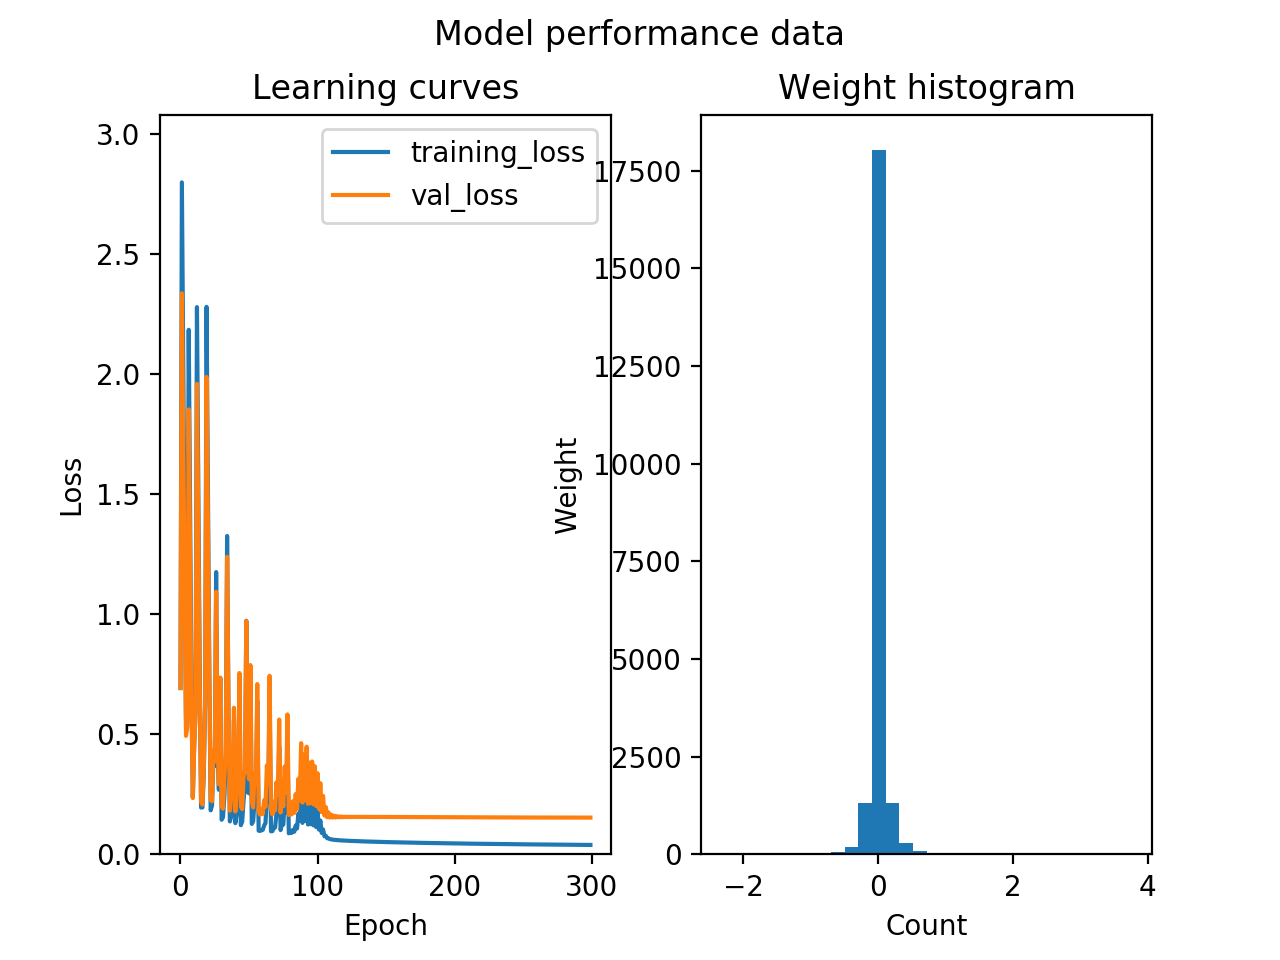
\includegraphics[width=\columnwidth, keepaspectratio]{{../results/12_300_softm_0.0001}.png}
    \caption{Learning Curve Showing High Learning Rate Will Stablize Despite Initial Vibrations}
    \label{fig:learning_rate}
\end{figure}

I also tried to use other loss functions and weight decays. My own logistics loss function worked very similar to the built-in soft margin loss. In fact when the learning rate was low I can get identical scores on both loss funcitons but when the learning rate went up, e.g. \verb|learning_rate=3| my logistics loss function performed worse than the soft margin one by 10\%. Other loss functions were bad as well even when running with their best set of hyperparameters. Weight decay can shorten the distance between the training data performance and the validation data one but it didn't help grow the accuracy and the F1-score.

In conclusion, my best set of hyperparameters for now are listed below. They help me achieve 0.937 of accuracy and 0.424 of F1-score on the validation data set.

\begin{lstlisting}[language=Python]
    learning_rate = 12
    epoches = 300
    loss_function = torch.nn.SoftMarginLoss()
    weight_decay = 0.0001
\end{lstlisting}

Both of the top 10 features from the classifier make sense to English speakers, especially the positive one. Words such as ``stupid'', ``fuck'' and ``dumb'' are clearly signs of discussions went off rail. In the negative features ``='' is the one with lowest weight. Wikipedia uses ``='' very often in their markup language hence this can be the interpreted that people are describing a bug or a web page formatting issue rather than the content, which is more rational and less emotional since they are showing each other the actual code. Other words in the negative features like ``might'', ``Thank'' etc. are typical words in English to express uncertainty (to suggest opposite opinions politely) and grateful.

\section{Testing and Reflection}

For the moment my classifier can't generalize its knowledge to the test data very well. I can achieve 0.945 of accuracy and 0.56 of F1-score on the test data, which is roughly at the same level with the performance on the validation data. But comparing them with the training data set that has an F1-score of 0.96 they are both way off the target. This is mainly caused by the low recall (below 0.3) which means our predictions can only pickup half of the true positives, or in another word the true personal attack words.

But there are definitely ways to improve. For example choosing \verb|Adam| instead of \verb|SGD| to be our optimizer. However the real challenge is to figure out an efficient solution to the highly skewed data set. I have seen lots of discussions on the internet that suggest people trying \verb|BCELoss()| or \verb|BCEWithLogitsLoss()| as the loss function\footnote{\url{https://discuss.pytorch.org/t/dealing-with-imbalanced-datasets-in-pytorch/22596/11}}. After some tweaks like relabeling the negative sample to 0 instead 1 and giving a higher weight to the positive labels, I have improved the the F1 score on the test data set to 0.634.

In addition some other posts mentioned oversampling/undersampling some classes as well. In our data set I think by oversampling those positive data should be the option to help countact data skewness. \verb|PyTorch| has some built-in utilities for sampling data\footnote{\url{https://pytorch.org/docs/stable/data.html?highlight=dataloader#torch.utils.data.DataLoader}} so definitely it is feasible.

Overall, developing using libraries specialized in matrix or vector processing saves a lot of time from tedious array operations and calculations, but users are required to change their minds to think about the question and the formulas in vector spaces. Besides that, \verb|PyTorch| has plenty of everyday-using functions for machine learning to call and a large community of users to discuss with. It is easier for actual engineering problems, though it can lead people to concern less on the theoratical part.

\section{Minibatch Training}

Minibatch means the training data is feeded into the classifier in small batches instead. Luckily in \verb|util2.py| I saw the \verb|SentimentData| class already has a random slice function called \verb|random_split()|, it's OK to do our work after understanding the magic behind and fix a bug inside at calling \verb|self._split_data()|. Also reuse that function is way more easier than the standard \verb|PyTorch DataLoader()| way. Then I just splited the training data and its labels into 2 arrays before the dense representation tranformation (I used to do that inside the training loop but that can be super slow).

The result, from my experience, didn't improve the accuracy or the F1-score a lot. But the best thing of it is that now the model converge much faster at the same learning rate. For example when learning rate was at 0.001 and epoch was 300, the tranditional Stochastic Gradient Descent way hasn't started to converge even at the end of training, but minibatch training can converge just passed around 50-60 epoches. Hence although for each epoch the calculation time is longer but thanks to the shorter epoches the whole training time can still be saved.

The parameter, \verb|batch_size| will affect the performance a lot. On one hand the larger the batch size is the longer it takes in every epoch to calculate. But I can also see the accuracy and the F1-score increase with the batch size until 64. When \verb|batch_size=1| the classifier will behave exactly like the original one, which updates itself after each training sample.

\section{Checkpointing\textbackslash Early Stopping}

The time it takes to reach the best model and the best value of the $p$ patience parameter depends on the character of the model. For example when I am using the minibatch optimizer, since it will converge fast I am confident to give it a low patience number, but on the tranditional non-minibatch optimizer I need to increase the patience as it takes more time to converge. Anyway in both cases the pre-requirement is that the learning rate is in a reasonable range. It is neither too small which makes the learning curve converge slow, nor too big so the learning curve will never converge.

Also different models show different speeds in converging. Minibatch models converge in 20-30 epoches, but the non-minibatch ones converge at around 100 epoches.

\end{document}
